\chapter{Les échanges gazeux respiratoires}\label{ch:b1:gas-exchange}

Un litre d'air contient trente fois plus d'oxygène qu'un litre d'eau,
pèse huit cents fois moins, et laisse l'oxygène y diffuser dix mille
fois plus vite. Une truite doit faire passer cent cinquante grammes
d'eau sur ses \omterm{def:b1:gas-exchange:gill}{branchies} pour chaque milligramme d'oxygène qu'elle
prélève, et elle extrait les quatre cinquièmes de ce que l'eau
transporte~; un humain déplace quelques grammes d'air par milligramme
et en gaspille les trois quarts. Les deux \omterm{def:b1:mammal-organization:organ}{organes} sont deux réponses à
une même équation --- le flux d'un gaz à travers une surface --- dans
deux milieux. Ce chapitre énonce la physique, en déduit ce que doit
être une \omterm{prop:b1:organism-environment:surfaces}{surface d'échange}, décrit \omterm{def:b1:gas-exchange:gill}{branchies}, \omterm{def:b1:gas-exchange:lung}{poumons} et trachées,
suit l'oxygène et le dioxyde de carbone dans le sang, et examine le
contrôle de la ventilation, l'altitude et la plongée.

\section{La physique d'un gaz dans deux milieux}

\begin{definition}[Pression partielle, solubilité]\label{def:b1:gas-exchange:partial}
\index{pression partielle}
Dans un mélange de gaz, chaque gaz exerce une \emph{pression
partielle} proportionnelle à sa fraction~: dans l'air à \qty{101}{kPa},
l'oxygène (\qty{20.9}{\%}) a $P_{\mathrm{O_2}} = \qty{21.2}{kPa}$, le
dioxyde de carbone (\qty{0.04}{\%}) \qty{0.04}{kPa}. Un gaz se dissout
dans un liquide proportionnellement à sa pression partielle (loi de
Henry)~: l'eau en équilibre avec l'air à \qty{15}{\celsius} contient
\qty{0.32}{mmol/L} d'oxygène (\qty{10}{mg/L}, \qty{7}{mL/L} de gaz),
contre \qty{8.7}{mmol/L} (\qty{210}{mL/L}) dans l'air lui-même. La
pression partielle --- la même dans l'eau et dans l'air à l'équilibre
--- est ce qui entraîne la diffusion entre milieux~; le contenu est ce
qu'un respirateur peut extraire. Le dioxyde de carbone est vingt-cinq
fois plus soluble que l'oxygène~: il n'est jamais le gaz difficile.
\end{definition}

\begin{theorem}[Loi de Fick pour une surface d'échange]\label{thm:b1:gas-exchange:fick}
\index{loi de Fick}
La vitesse à laquelle un gaz traverse une membrane d'aire $A$ et
d'épaisseur $x$ séparant deux milieux aux \omterm{def:b1:gas-exchange:partial}{pressions partielles} $P_1$ et $P_2$ vaut
\[
\dot V = K\,\frac{A}{x}\,(P_1 - P_2),
\]
où $K$, la constante de diffusion (constante de Krogh) de la membrane,
combine la diffusivité et la solubilité du gaz dans le \omterm{def:b1:body-plans-tissues:tissue}{tissu}. Le flux
est augmenté par une aire plus grande, une barrière plus mince et une
différence de \omterm{def:b1:gas-exchange:partial}{pression partielle} plus forte~; rien d'autre.
\end{theorem}
\begin{proof}
La première \omterm{thm:b1:membranes-transport:fick}{loi de Fick} appliquée au gaz dissous dans la membrane
(\cref{ch:b1:membranes-transport}) donne un flux par unité d'aire
proportionnel au gradient de concentration~; par la loi de Henry, la
concentration à chaque face est proportionnelle à la \omterm{def:b1:gas-exchange:partial}{pression
partielle} du milieu qui la borde, de sorte que le gradient vaut
$(P_1 - P_2)/x$ fois la solubilité, et la constante absorbe
solubilité et diffusivité.
\end{proof}

\begin{omfigure}
\begin{tikzpicture}
\begin{axis}[
  ybar, bar width=16pt,
  width=0.72\linewidth, height=5.6cm,
  axis x line=bottom, axis y line=left,
  ymode=log, log origin=infty, ymin=0.1, ymax=3000,
  ylabel={oxygène par litre de milieu (\unit{mL})},
  ylabel style={font=\small},
  symbolic x coords={air, eau 5 C, eau 15 C, eau 30 C, eau de mer 15 C},
  xtick=data, x tick label style={font=\small, rotate=20, anchor=north east},
  enlarge x limits=0.15,
  nodes near coords, nodes near coords style={font=\scriptsize, anchor=south},
  point meta=rawy,
]
\addplot[fill=omDef!45, draw=omDef] coordinates {(air,210) (eau 5 C,9.0) (eau 15 C,7.1) (eau 30 C,5.3) (eau de mer 15 C,5.8)};
\end{axis}
\end{tikzpicture}

{\small Teneur en oxygène de l'air et de l'eau en équilibre avec lui.
L'eau en contient trente fois moins, et moins encore lorsqu'elle est
chaude ou salée~: un poisson dans un étang d'été vit au bord de la
pénurie.}
\end{omfigure}

\begin{proposition}[Ce que doit être une surface d'échange]\label{prop:b1:gas-exchange:requirements}
\index{surface d'echange@surface d'échange}
Un \omterm{def:b1:organism-environment:organism}{organisme} de plus d'un millimètre ne peut être approvisionné par
diffusion à travers sa surface externe
(\cref{ch:b1:organism-environment}). Il lui faut une \emph{surface
respiratoire} vaste (pour augmenter $A$), mince (pour abaisser $x$),
humide (les gaz ne traversent les membranes qu'en solution),
\emph{ventilée} --- le milieu externe renouvelé, pour que $P_1$ reste
élevée --- et \emph{perfusée} --- le sang qui la borde renouvelé, pour
que $P_2$ reste basse~; et une circulation qui porte le gaz de la
surface aux \omterm{def:b1:body-plans-tissues:tissue}{tissus}. \omterm{def:b1:gas-exchange:gill}{Branchies}, \omterm{def:b1:gas-exchange:lung}{poumons} et trachées sont trois façons
de replier une telle surface dans un corps et d'y faire circuler les
deux fluides.
\end{proposition}

\section{Les branchies et le contre-courant}

\begin{definition}[Branchie]\label{def:b1:gas-exchange:gill}
\index{branchie}
Une \emph{branchie} est une évagination de la surface du corps dans
l'eau, repliée en filaments et en \emph{lamelles} épaisses de quelques
micromètres, que le sang parcourt dans des capillaires. Les branchies
d'un poisson pendent de quatre arcs osseux de chaque côté~; l'eau
aspirée par la bouche et refoulée sous les opercules par un système à
deux \omterm{def:b1:membranes-transport:transporters}{pompes} circule entre les lamelles dans un sens, et le sang dans
les lamelles circule dans l'autre~: un
\emph{contre-courant}\index{echange a contre-courant@échange à contre-courant}. Une truite d'un
kilogramme possède quelque \qty{2000}{cm^2} de surface lamellaire,
épaisse de \qty{2}{\micro m}.
\end{definition}

\begin{omfigure}
\begin{tikzpicture}
  \node[anchor=south west, inner sep=0] (img) at (0,0)
    {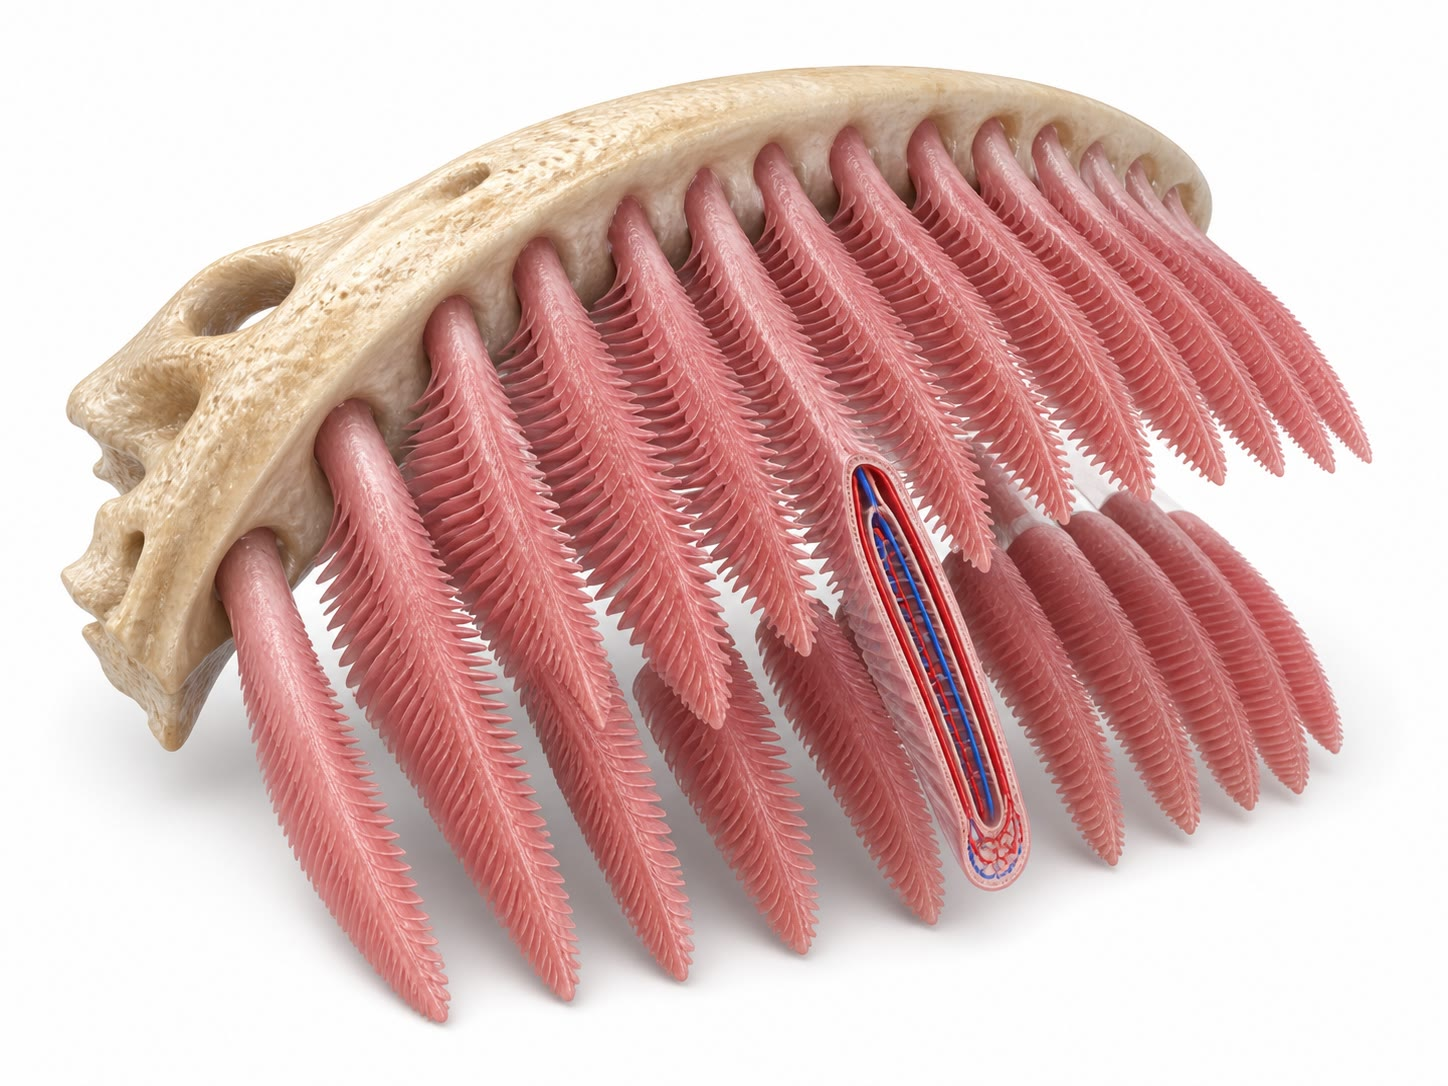
\includegraphics[width=0.52\linewidth]{images/book3/ai/fig-gill-lamellae.jpg}};
  \begin{scope}[x={(img.south east)}, y={(img.north west)},
      every node/.style={font=\small}]
    \draw[omDef, thick] (0.20,0.50) -- (-0.03,0.60) node[left] {arc branchial};
    \draw[omDef, thick] (0.55,0.70) -- (0.55,1.08) node[above] {filaments};
    \draw[omDef, thick] (0.75,0.40) -- (1.03,0.30) node[right, align=left] {lamelles~: la surface\\ d'échange, \qty{2}{\micro m}};
    \draw[omDef, thick] (0.45,0.20) -- (0.45,-0.08) node[below] {vaisseaux sanguins le long du filament};
  \end{scope}
\end{tikzpicture}

{\small Un arc branchial avec ses filaments et leurs lamelles. L'eau
circule entre les lamelles~; le sang les traverse en sens inverse.}
\end{omfigure}

\begin{theorem}[Échange à contre-courant]\label{thm:b1:gas-exchange:countercurrent}
Lorsque l'eau et le sang circulent en sens opposés le long d'une
\omterm{prop:b1:organism-environment:surfaces}{surface d'échange}, le sang qui quitte la \omterm{def:b1:gas-exchange:gill}{branchie} peut approcher la
\omterm{def:b1:gas-exchange:partial}{pression partielle} de l'eau qui y \emph{entre}, et l'eau peut être
dépouillée de la plus grande part de son oxygène~: des extractions de
\qty{80}{\%} ou plus. S'ils circulent dans le même sens (co-courant),
les deux fluides convergent vers une valeur intermédiaire commune et
l'extraction ne peut dépasser \qty{50}{\%}.
\end{theorem}
\begin{proof}
Le long d'un échangeur à co-courant, la différence $P_{\text{eau}} -
P_{\text{sang}}$ décroît de sa valeur d'entrée jusqu'à zéro à mesure
que les deux se rapprochent d'une même pression~; une fois égales,
plus aucun gaz ne passe, et pour des débits égaux le point de
rencontre est à mi-chemin. En \omterm{def:b1:gas-exchange:gill}{contre-courant}, le sang, en avançant
vers sa sortie, rencontre une eau toujours plus fraîche, si bien
qu'une différence positive est maintenue sur toute la longueur~: le
sang, à sa sortie, fait face à l'eau entrante à \qty{21}{kPa}, et
l'eau, à sa sortie, au sang veineux entrant à quelques kilopascals.
La limite est fixée par la surface, non par un équilibre.
\end{proof}

\begin{omfigure}
\begin{tikzpicture}[font=\footnotesize, >=Stealth, line cap=round]
  % co-current
  \begin{scope}
    \node[anchor=south, font=\small] at (2.6,1.65) {co-courant~: les deux flux dans le même sens};
    \draw[->, very thick, omDef] (0,1.2) -- (5.2,1.2) node[right] {eau sortante~: \qty{12}{kPa}};
    \draw[->, very thick, omThm] (0,0.4) -- (5.2,0.4) node[right] {sang sortant~: \qty{12}{kPa}};
    \node[anchor=east, omDef] at (-0.1,1.2) {eau entrante~: \qty{21}{kPa}};
    \node[anchor=east, omThm] at (-0.1,0.4) {sang entrant~: \qty{3}{kPa}};
    \foreach \x/\d in {0.6/18, 1.6/12, 2.6/7, 3.6/3, 4.6/0.5} { \draw[->, gray] (\x,1.05) -- (\x,0.55) node[midway, right, font=\scriptsize, gray] {\d}; }
    \node[anchor=north, align=center] at (2.6,0.1) {la différence (en gris, kPa) tombe à zéro~:\\ l'extraction s'arrête à \qty{43}{\%}};
  \end{scope}
  \begin{scope}[yshift=-3.6cm]
    \node[anchor=south, font=\small] at (2.6,1.65) {contre-courant~: flux opposés};
    \draw[->, very thick, omDef] (0,1.2) -- (5.2,1.2) node[right] {eau sortante~: \qty{4}{kPa}};
    \draw[<-, very thick, omThm] (0,0.4) -- (5.2,0.4) node[right] {sang entrant~: \qty{3}{kPa}};
    \node[anchor=east, omDef] at (-0.1,1.2) {eau entrante~: \qty{21}{kPa}};
    \node[anchor=east, omThm] at (-0.1,0.4) {sang sortant~: \qty{18}{kPa}};
    \foreach \x/\d in {0.6/3, 1.6/3, 2.6/3, 3.6/3, 4.6/2} { \draw[->, gray] (\x,1.05) -- (\x,0.55) node[midway, right, font=\scriptsize, gray] {\d}; }
    \node[anchor=north, align=center] at (2.6,0.1) {la différence reste positive tout du long~:\\ l'extraction atteint \qty{80}{\%}, le sang sort près de la valeur d'entrée de l'eau};
  \end{scope}
\end{tikzpicture}

{\small Échange à co-courant et à \omterm{def:b1:gas-exchange:gill}{contre-courant}, à surface et débits
égaux. Opposer les flux maintient un gradient sur toute la longueur et
laisse le sang approcher la pression d'oxygène de l'eau fraîche.}
\end{omfigure}

\begin{omfigure}
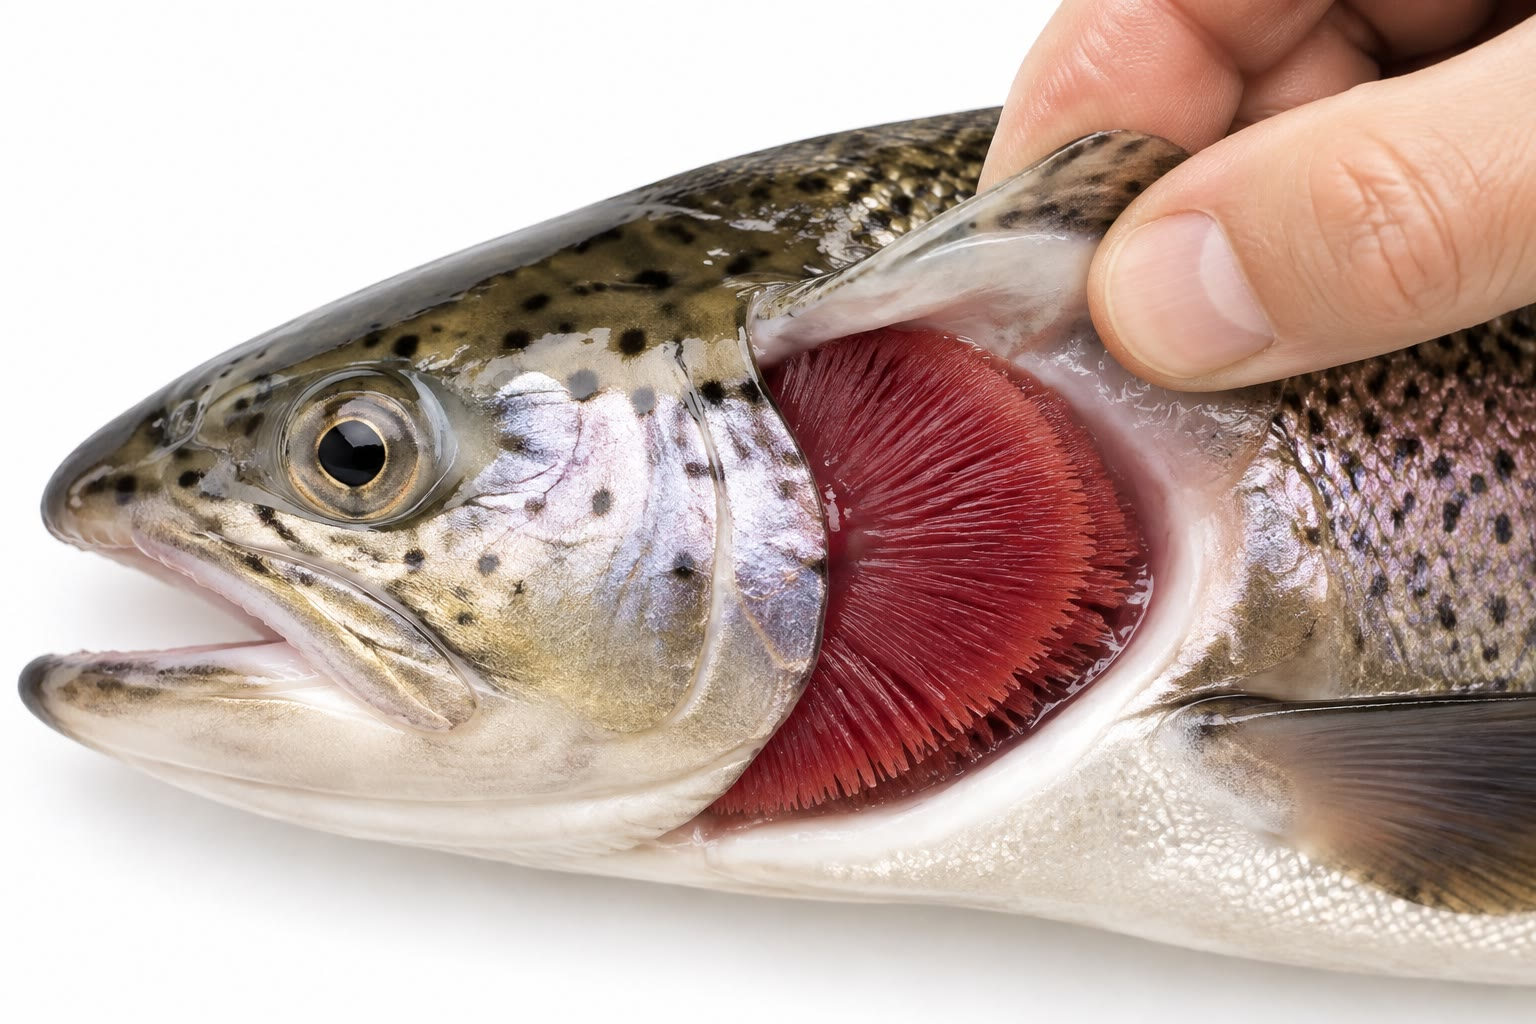
\includegraphics[width=0.5\linewidth]{images/book3/ai/b3-21-trout-gills.jpg}

{\small Les \omterm{def:b1:gas-exchange:gill}{branchies} d'une truite sous l'opercule soulevé~: rouges de
sang, parce que les lamelles ont deux \omterm{def:b1:cell-unit-of-life:cell}{cellules} d'épaisseur et que le
sang est à un micromètre de l'eau.}
\end{omfigure}

\begin{example}[Le prix de l'eau]\label{ex:b1:gas-exchange:priceofwater}
Une truite de \qty{1}{kg} au repos prélève environ \qty{50}{mL}
d'oxygène par heure. À partir d'une eau à \qty{7}{mL/L}, avec
\qty{80}{\%} d'extraction, elle doit pomper \qty{9}{L} d'eau par heure
sur ses \omterm{def:b1:gas-exchange:gill}{branchies} --- neuf kilogrammes d'un milieu cinquante fois plus
visqueux que l'air, à travers des canaux larges d'une fraction de
millimètre. Un dixième de son métabolisme part dans la respiration~;
un humain au repos y consacre un cinquantième. Réchauffez l'étang à
\qty{30}{\celsius} et le même poisson, qui a besoin de plus d'oxygène
d'une eau qui en contient moins, devra pomper trois fois plus.
\end{example}

\section{Respirer l'air~: poumons et trachées}

\begin{definition}[Le poumon des mammifères]\label{def:b1:gas-exchange:lung}
\index{poumon}\index{alveole@alvéole}
Un \emph{poumon} est une invagination de la surface du corps dans une
chambre interne humide, qui garde la surface mouillée en air sec. Le
poumon des mammifères est un arbre de voies aériennes terminé par
quelque trois cents millions d'\emph{alvéoles}, sacs de \qty{0.2}{mm}
dont les parois --- une \omterm{def:b1:cell-unit-of-life:cell}{cellule} épithéliale et un endothélium
capillaire, \qty{0.5}{\micro m} en tout --- totalisent \qty{100}{m^2}
chez l'humain, enveloppées d'un réseau capillaire que traverse tout le
débit cardiaque. Il est ventilé de façon \emph{alternante}~: le
\omterm{def:b1:mammal-organization:bodyplan}{diaphragme} et les muscles intercostaux élargissent le thorax, l'air
entre~; ils se relâchent, l'air ressort par le même chemin. Une
inspiration déplace \qty{500}{mL}, dont \qty{150}{mL} ne remplissent
que les voies aériennes (\emph{espace mort}) et n'atteignent jamais
une alvéole~; le gaz alvéolaire, renouvelé d'un septième à chaque
souffle, reste à $P_{\mathrm{O_2}} =
\qty{13.3}{kPa}$ et $P_{\mathrm{CO_2}} = \qty{5.3}{kPa}$ --- les
pressions avec lesquelles le sang s'équilibre.
\end{definition}

\begin{omfigure}
\begin{tikzpicture}
  \node[anchor=south west, inner sep=0] (img) at (0,0)
    {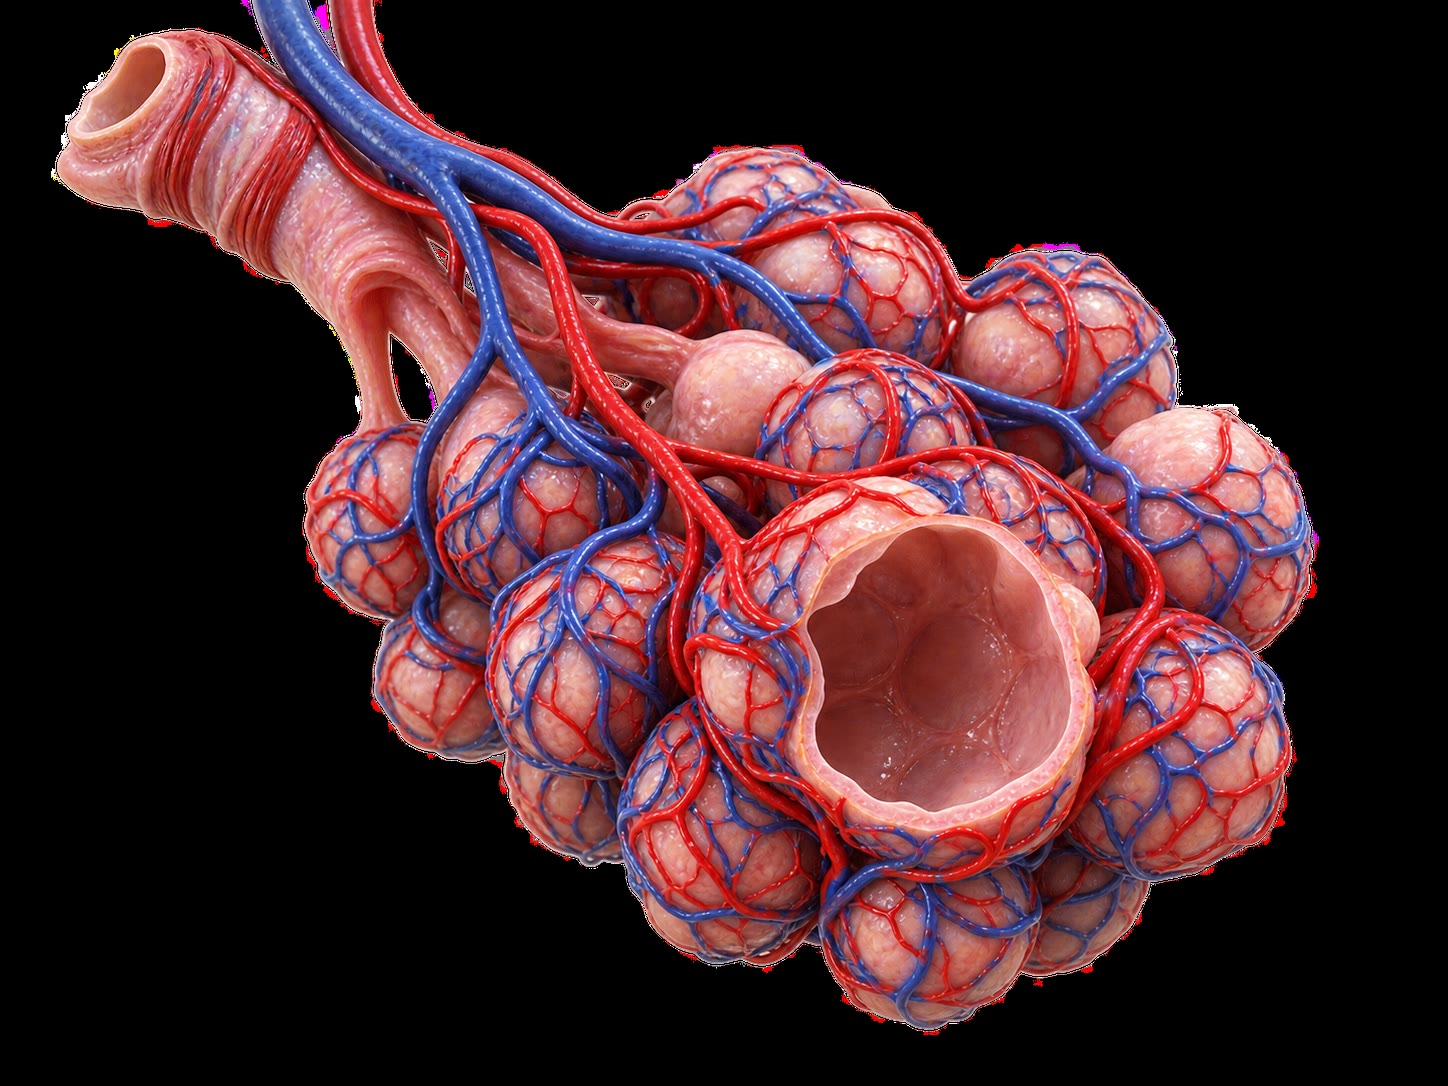
\includegraphics[width=0.5\linewidth]{images/book3/ai/fig-alveoli.jpg}};
  \begin{scope}[x={(img.south east)}, y={(img.north west)},
      every node/.style={font=\small}]
    \draw[omDef, thick] (0.50,0.85) -- (0.50,1.08) node[above] {voie aérienne terminale};
    \draw[omDef, thick] (0.30,0.45) -- (-0.03,0.40) node[left, align=right] {alvéole ouverte~:\\ l'air à l'intérieur};
    \draw[omDef, thick] (0.75,0.55) -- (1.03,0.62) node[right, align=left] {réseau capillaire\\ sur la paroi};
    \draw[omDef, thick] (0.60,0.15) -- (0.60,-0.08) node[below] {paroi~: \qty{0.5}{\micro m} entre l'air et le sang};
  \end{scope}
\end{tikzpicture}

{\small Des \omterm{def:b1:gas-exchange:lung}{alvéoles} au bout d'une voie aérienne, enveloppées de
capillaires. Tout le débit cardiaque s'étale sur cent mètres carrés de
cette paroi, une fraction de seconde à la fois.}
\end{omfigure}

\begin{proposition}[Trois architectures pour l'air]\label{prop:b1:gas-exchange:designs}
\index{trachees@trachées}
Les \emph{mammifères} ventilent de façon alternante~: simple, mais
l'air frais se mêle à l'air vicié, l'oxygène alvéolaire vaut les deux
tiers de celui de l'atmosphère et l'extraction est d'un quart. Les
\emph{oiseaux} font passer l'air dans un seul sens à travers de fins
tubes (parabronches) entre deux jeux de sacs aériens qui font office
de soufflets, de sorte que l'air frais traverse la \omterm{prop:b1:organism-environment:surfaces}{surface d'échange} à
l'inspiration comme à l'expiration, à courants croisés avec le sang~:
leur extraction est plus élevée, et l'oie à tête barrée survole
l'Himalaya où un mammifère s'évanouirait. Les \emph{insectes} n'ont
aucun sang respiratoire~: l'air entre par des valves (\emph{stigmates})
dans des \emph{trachées}, tubes raidis par des épaississements en
spirale qui se ramifient jusqu'au micromètre et livrent l'oxygène par
diffusion directement à chaque \omterm{def:b1:cell-unit-of-life:cell}{cellule}, avec l'aide de pompages de
l'abdomen chez les insectes grands ou actifs. La diffusion le long de
tubes limite cette architecture aux petits corps --- une des raisons
pour lesquelles aucun insecte n'est plus gros qu'une souris.
\end{proposition}

\begin{omfigure}
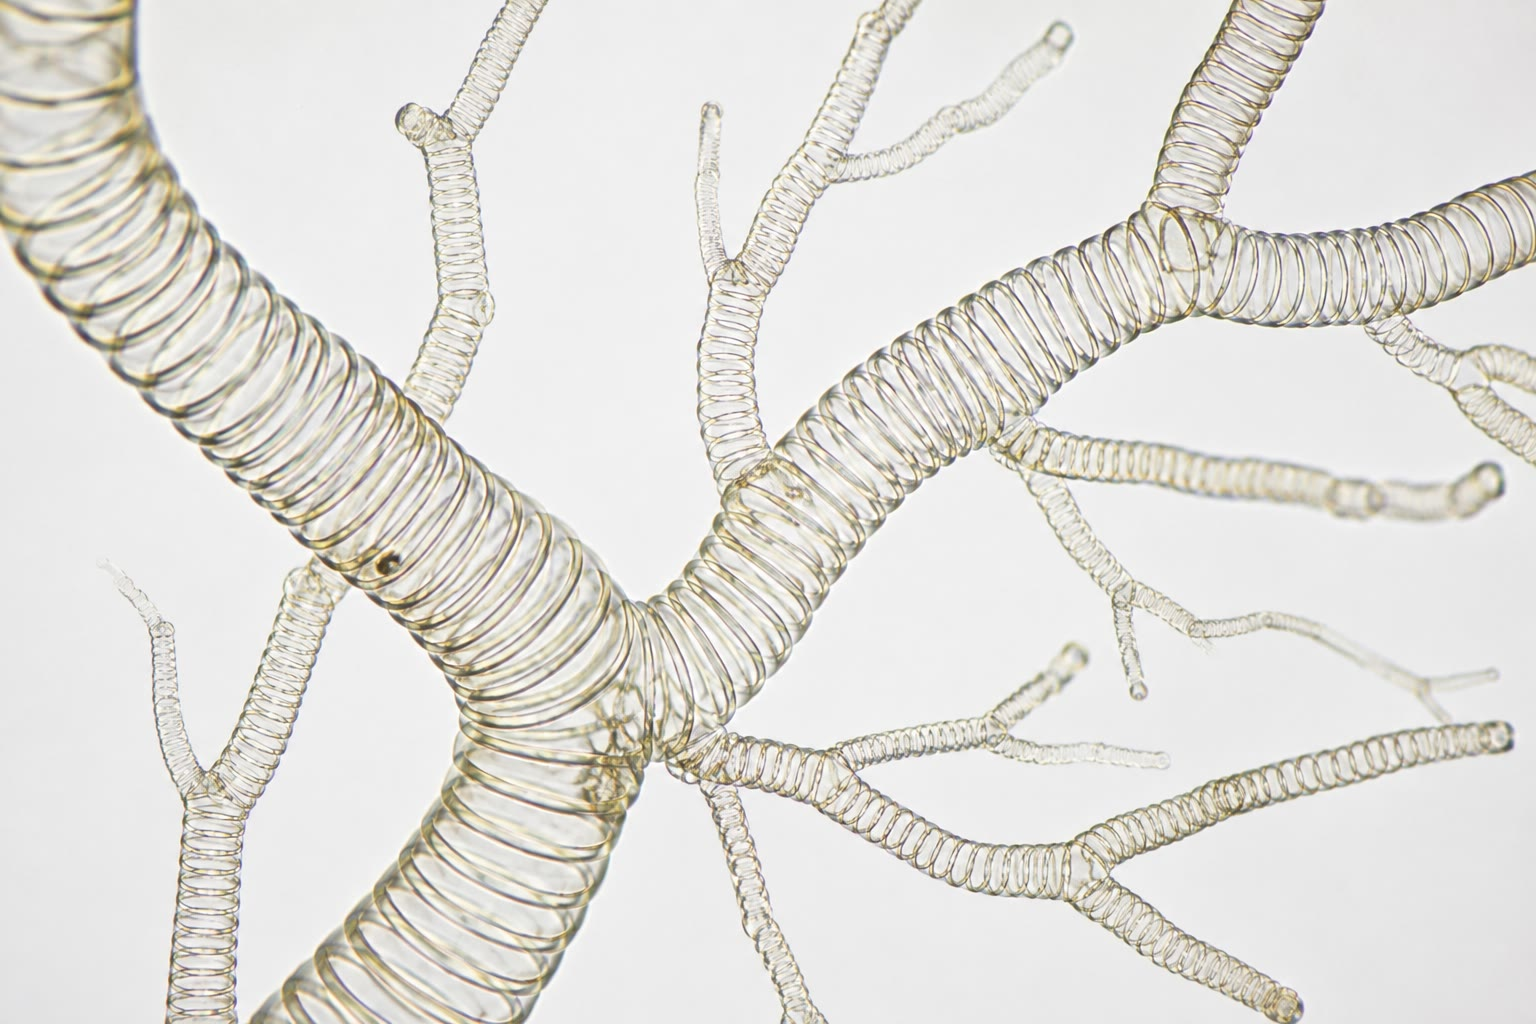
\includegraphics[width=0.5\linewidth]{images/book3/ai/b3-21-insect-tracheae.jpg}

{\small Trachées d'insecte~: des tubes remplis d'air maintenus ouverts
par des épaississements en spirale, ramifiés jusqu'aux \omterm{def:b1:cell-unit-of-life:cell}{cellules}. Aucun
sang ne porte l'oxygène~; l'air va jusqu'au bout.}
\end{omfigure}

\begin{method}[Lire un bilan ventilatoire]\label{met:b1:gas-exchange:budget}
\begin{enumerate}
  \item Ventilation minute $=$ volume courant $\times$ nombre de
        respirations par minute~; ventilation alvéolaire $=$ (volume
        courant $-$ espace mort) $\times$ nombre de respirations par
        minute. Seule la seconde échange du gaz.
  \item Consommation d'oxygène $=$ ventilation alvéolaire $\times$
        (fraction inspirée $-$ fraction alvéolaire)~; au repos,
        $\qty{4.2}{L/min}\times(0.21 - 0.14) \approx \qty{0.3}{L/min}$.
  \item Extraction $=$ consommation $/$ (ventilation $\times$ fraction
        inspirée)~: un quart dans un \omterm{def:b1:gas-exchange:lung}{poumon} à ventilation alternante,
        quatre cinquièmes dans une \omterm{def:b1:gas-exchange:gill}{branchie} à \omterm{def:b1:gas-exchange:gill}{contre-courant}.
  \item Du côté du sang~: consommation $=$ débit cardiaque $\times$
        (contenu artériel $-$ contenu veineux)~; \qty{5}{L/min}$\times$
        \qty{50}{mL/L} au repos, les mêmes \qty{250}{mL/min}. Les deux
        bilans doivent coïncider.
\end{enumerate}
\end{method}

\section{Les gaz dans le sang}

\begin{proposition}[Transport de l'oxygène et du dioxyde de carbone]\label{prop:b1:gas-exchange:transport}
\index{anhydrase carbonique}\index{effet Bohr}\index{effet Haldane}
Le \omterm{def:b1:mammal-organization:compartments}{plasma} ne dissout que \qty{3}{mL} d'oxygène par litre à la pression
artérielle~; l'hémoglobine (\cref{ch:b1:proteins}) en transporte
\qty{200}{mL}, chargée dans le \omterm{def:b1:gas-exchange:lung}{poumon} à \qty{13.3}{kPa} et en
déchargeant du cinquième à la moitié dans les \omterm{def:b1:body-plans-tissues:tissue}{tissus}. Le dioxyde de
carbone voyage de trois façons~: \qty{7}{\%} dissous, \qty{23}{\%} lié
aux groupements aminés de l'hémoglobine et \qty{70}{\%} sous forme de
bicarbonate~: dans l'hématie, l'\emph{\omterm{prop:b1:gas-exchange:transport}{anhydrase
carbonique}} transforme $\mathrm{CO_2}$ et eau en acide carbonique en
quelques millisecondes, l'acide se dissocie, le bicarbonate quitte la
\omterm{def:b1:cell-unit-of-life:cell}{cellule} en échange de chlorure (le \emph{déplacement des chlorures}) et
le proton est pris en charge par l'hémoglobine. Les deux gaz
s'entraident~: l'acidité et le
$\mathrm{CO_2}$ abaissent l'affinité de l'hémoglobine pour l'oxygène (\emph{\omterm{prop:b1:gas-exchange:transport}{effet
Bohr}}), donc l'oxygène est libéré là où le $\mathrm{CO_2}$ est produit~; et
l'hémoglobine désoxygénée fixe mieux protons et $\mathrm{CO_2}$
(\emph{\omterm{prop:b1:gas-exchange:transport}{effet Haldane}}), donc le $\mathrm{CO_2}$ est capté là où l'oxygène
est libéré, et rendu dans le \omterm{def:b1:gas-exchange:lung}{poumon} à mesure que l'oxygène se charge.
\end{proposition}

\begin{omfigure}
\begin{tikzpicture}[font=\footnotesize, >=Stealth, line cap=round]
  % red cell
  \draw[very thick, omThm!80!black, fill=omThm!8, rounded corners=18pt] (0,0) rectangle (7.6,4.0);
  \node[anchor=north west, omThm!80!black, font=\small] at (0.15,3.95) {hématie (dans un capillaire tissulaire)};
  % CO2 in from tissue
  \draw[->, very thick, omDef] (-1.6,2.6) -- (0,2.6) node[pos=0, left, align=right] {$\mathrm{CO_2}$ venant\\ du tissu};
  \node[draw, thick, fill=white, rounded corners=3pt, inner sep=2pt] (ca) at (2.0,2.6) {$\mathrm{CO_2} + \mathrm{H_2O} \to \mathrm{H_2CO_3}$};
  \node[anchor=south, font=\scriptsize, omProp!80!black] at (2.0,2.95) {anhydrase carbonique};
  \node[draw, thick, fill=white, rounded corners=3pt, inner sep=2pt] (dis) at (5.2,2.6) {$\mathrm{H^+} + \mathrm{HCO_3^-}$};
  \draw[->, thick] (ca) -- (dis);
  % bicarbonate out, chloride in
  \draw[->, very thick, omDef] (6.2,2.4) -- (6.2,0.9) -- (8.4,0.9) node[right, align=left] {$\mathrm{HCO_3^-}$ vers le plasma\\ (\qty{70}{\%} du $\mathrm{CO_2}$)};
  \draw[<-, very thick, gray] (6.9,1.85) -- (8.4,1.85) node[right, gray] {$\mathrm{Cl^-}$ en échange};
  % proton to Hb, O2 release
  \node[draw, thick, fill=omThm!25, rounded corners=3pt, inner sep=2pt] (hb) at (4.0,1.0) {hémoglobine};
  \draw[->, thick] (4.7,2.35) -- (4.2,1.3) node[midway, right, font=\scriptsize] {$\mathrm{H^+}$ fixé};
  \draw[->, very thick, omExo!70!black] (hb.west) -- (0,1.0) -- (-1.6,1.0) node[left, align=right] {$\mathrm{O_2}$ libéré\\ (effet Bohr)};
  \node[anchor=north, align=center, gray] at (3.8,-0.2) {dans le poumon chaque flèche s'inverse~: l'oxygène se charge, protons et $\mathrm{CO_2}$ sont libérés,\\ le bicarbonate revient dans la cellule et le $\mathrm{CO_2}$ est expiré};
\end{tikzpicture}

{\small Le dioxyde de carbone dans une hématie. L'\omterm{prop:b1:gas-exchange:transport}{anhydrase carbonique}
fabrique l'acide carbonique~; le bicarbonate part vers le \omterm{def:b1:mammal-organization:compartments}{plasma} et le
proton est pris par l'hémoglobine, qui libère l'oxygène en le fixant.}
\end{omfigure}

\begin{example}[Un litre de sang dans un muscle au travail]\label{ex:b1:gas-exchange:litre}
Le sang artériel apporte \qty{200}{mL} d'oxygène par litre et
\qty{480}{mL} de dioxyde de carbone (surtout en bicarbonate). Dans un
muscle au repos, il y laisse \qty{50}{mL} d'oxygène et prend
\qty{40}{mL} de $\mathrm{CO_2}$~; le pH veineux ne baisse que de
\qty{0.04}{}, parce que l'hémoglobine a absorbé les protons. Dans un
muscle qui sprinte, à pH 7,2 et $P_{\mathrm{O_2}}$ de \qty{2.7}{kPa},
le même litre y laisse \qty{150}{mL} d'oxygène
(\cref{ch:b1:proteins}) et emporte aussi le lactate.
\end{example}

\section{Contrôle, altitude et plongée}

\begin{proposition}[La ventilation est contrôlée par le dioxyde de carbone]\label{prop:b1:gas-exchange:control}
\index{chimiorecepteur@chimiorécepteur}
Le rythme respiratoire est engendré dans le tronc cérébral et ajusté
par des \emph{chimiorécepteurs}~: les centraux, baignés par le liquide
qui entoure le cerveau, répondent au changement de pH que produit le
$\mathrm{CO_2}$~; les périphériques, dans les artères carotides,
répondent à une chute de l'oxygène artériel au-dessous de
\qty{8}{kPa} environ. Dans la vie ordinaire, c'est le
$\mathrm{CO_2}$ qui commande~: une hausse de \qty{1}{kPa} de la
$P_{\mathrm{CO_2}}$ artérielle double à peu près la ventilation, alors que
l'oxygène doit chuter d'un tiers avant qu'elle ne réponde. Retenir son
souffle finit quand le
$\mathrm{CO_2}$, et non l'oxygène, atteint la limite~; hyperventiler d'abord
abaisse le $\mathrm{CO_2}$ et laisse un plongeur rester sous l'eau jusqu'à
épuisement de l'oxygène --- inconscient avant que l'envie de respirer
ne revienne.
\end{proposition}

\begin{omfigure}
\begin{tikzpicture}
\begin{axis}[
  width=0.86\linewidth, height=5.8cm,
  axis x line=bottom, axis y line=left,
  xmin=4, xmax=8.5, ymin=0, ymax=45,
  xlabel={$P_{\mathrm{CO_2}}$ artérielle (\unit{kPa})}, ylabel={ventilation (\unit{L/min})},
  xlabel style={font=\small, at={(axis description cs:0.5,-0.13)}, anchor=north},
  ylabel style={font=\small},
  tick label style={font=\small}, xtick={4,5,6,7,8}, ytick={0,10,20,30,40},
  legend style={font=\small, at={(0.03,0.97)}, anchor=north west, draw=none},
  clip=false,
]
\addplot[very thick, omDef, domain=4.5:8.5, samples=20] {6 + 10*(x-5.3)};
\addlegendentry{oxygène normal}
\addplot[very thick, omThm, domain=4.5:7.2, samples=20] {6 + 20*(x-5.3)};
\addlegendentry{oxygène bas (\qty{7}{kPa})~: plus raide}
\draw[dashed, gray] (axis cs:5.3,0) -- (axis cs:5.3,6); \node[font=\scriptsize, anchor=west] at (axis cs:5.4,1.5) {valeur de repos};
\end{axis}
\end{tikzpicture}

{\small Ventilation en fonction du dioxyde de carbone artériel. Chaque
kilopascal au-dessus de la valeur de repos ajoute environ
\qty{10}{L/min}~; un oxygène bas rend la réponse plus raide mais, seul,
ne fait pas grand-chose tant qu'il n'est pas très bas.}
\end{omfigure}

\begin{example}[Altitude et profondeur]\label{ex:b1:gas-exchange:altitudediving}
À \qty{4000}{m}, l'air contient \qty{12}{kPa} d'oxygène et les
\omterm{def:b1:gas-exchange:lung}{alvéoles} \qty{7}{}~: les corpuscules carotidiens poussent la
ventilation, ce qui chasse le $\mathrm{CO_2}$ et alcalinise le sang ---
un frein que les reins lèvent en quelques jours en excrétant du
bicarbonate~; les hématies élèvent leur BPG en quelques jours et la
moelle élève l'hémoglobine en quelques semaines
(\cref{ch:b1:proteins}). Un phoque qui plonge vingt minutes fait
l'inverse~: il expire avant de plonger, ralentit son cœur au dixième,
coupe le sang de tout sauf du cerveau et du cœur, et fait tourner ses
muscles sur l'oxygène fixé à leur propre myoglobine, dix fois plus
concentrée que la nôtre, puis sur la \omterm{def:b1:respiration-fermentation:fermentation}{fermentation}, en tolérant un
lactate que le corps épure en surface. Ses \omterm{def:b1:gas-exchange:lung}{poumons} s'affaissent
au-dessous de \qty{50}{m}, ce qui garde l'azote hors de son sang.
\end{example}

\section{Exercices}

\begin{exercise}[$\star$]\label{exo:b1:gas-exchange:1}
Énoncer la \omterm{thm:b1:membranes-transport:fick}{loi de Fick} pour une \omterm{prop:b1:organism-environment:surfaces}{surface d'échange} et citer les quatre
caractères qui augmentent le flux.
\end{exercise}

\begin{exercise}[$\star$]\label{exo:b1:gas-exchange:2}
Expliquer pourquoi l'eau est un milieu plus difficile à respirer que
l'air, en s'appuyant sur trois nombres.
\end{exercise}

\begin{exercise}[$\star$]\label{exo:b1:gas-exchange:3}
À partir de la figure du \omterm{def:b1:gas-exchange:gill}{contre-courant}, lire la pression d'oxygène de
l'eau sortante et du sang sortant dans chaque disposition, ainsi que
l'extraction.
\end{exercise}

\begin{exercise}[$\star$]\label{exo:b1:gas-exchange:4}
Sous quelles trois formes le dioxyde de carbone est-il transporté dans
le sang, et dans quelles proportions~?
\end{exercise}

\begin{exercise}[$\star\star$]\label{exo:b1:gas-exchange:5}
Une personne respire \qty{15}{} fois par minute avec un volume courant
de \qty{450}{mL} et un espace mort de \qty{150}{mL}. Calculer les
ventilations minute et alvéolaire, puis la consommation d'oxygène si
la fraction alvéolaire est de \qty{14}{\%}. Reprendre pour \qty{30}{}
respirations superficielles de \qty{225}{mL}.
\end{exercise}

\begin{exercise}[$\star\star$]\label{exo:b1:gas-exchange:6}
Un bocal à poisson rouge à \qty{25}{\celsius} contient \qty{6}{mL}
d'oxygène par litre. Un poisson de \qty{20}{g} consomme \qty{2}{mL}
d'oxygène par heure. Quel volume d'eau doit traverser ses \omterm{def:b1:gas-exchange:gill}{branchies}
par heure à \qty{75}{\%} d'extraction, et combien de fois son propre
volume cela représente-t-il~?
\end{exercise}

\begin{exercise}[$\star\star$]\label{exo:b1:gas-exchange:7}
Un \omterm{def:b1:gas-exchange:lung}{poumon} de \qty{100}{m^2} et \qty{0.5}{\micro m} transfère
\qty{250}{mL/min} sous une différence de pression moyenne de
\qty{8}{kPa}. Une maladie épaissit la paroi à \qty{2}{\micro m} et
divise l'aire par deux. Calculer le transfert sous la même différence,
et la différence nécessaire pour rétablir \qty{250}{mL/min}. Pourquoi
le corps ne peut-il pas simplement augmenter la différence~?
\end{exercise}

\begin{exercise}[$\star\star$]\label{exo:b1:gas-exchange:8}
Expliquer le déplacement des chlorures~: pourquoi le bicarbonate quitte
l'hématie, pourquoi le chlorure y entre, et ce qu'il adviendrait du
volume de la \omterm{def:b1:cell-unit-of-life:cell}{cellule} sans cet échange.
\end{exercise}

\begin{exercise}[$\star\star$]\label{exo:b1:gas-exchange:9}
Pourquoi un plongeur qui hyperventile avant une apnée risque-t-il la
noyade, alors que celui qui ne le fait pas remonte sain et sauf, mal à
l'aise mais conscient~?
\end{exercise}

\begin{exercise}[$\star\star\star$]\label{exo:b1:gas-exchange:10}
Une trachée d'insecte longue de \qty{1}{mm} et large de
\qty{20}{\micro m} alimente un muscle qui consomme \qty{1e-9}{mol}
d'oxygène par seconde. Avec $D = \qty{2e-5}{m^2/s}$ dans l'air et
\qty{8.7}{mol/m^3} d'oxygène au stigmate, calculer la concentration au
bout musculaire (Fick~: $J = DA\,\Delta c/L$). Reprendre pour une
trachée longue de \qty{10}{mm}. Qu'est-ce qui limite la taille des
insectes~?
\end{exercise}

\begin{exercise}[$\star\star\star$]\label{exo:b1:gas-exchange:11}
Les oiseaux et les poissons utilisent tous deux des flux non
alternants. Comparer leurs échangeurs (sens du milieu, relation au
flux sanguin, extraction) et expliquer pourquoi un \omterm{def:b1:gas-exchange:lung}{poumon} alternant ne
peut atteindre leur extraction, quelle que soit sa surface.
\end{exercise}

\begin{exercise}[$\star\star\star$]\label{exo:b1:gas-exchange:12}
«~Le \omterm{def:b1:gas-exchange:lung}{poumon} est réglé par le gaz qu'il excrète, non par celui qu'il
prélève.~» Discuter en un paragraphe~: pourquoi le $\mathrm{CO_2}$ est le
meilleur signal au niveau de la mer, quand la disposition échoue, et
comment l'altitude le révèle.
\end{exercise}

\section{Problème~: une truite et un humain}

\begin{problem}[{Problème du week-end --- une branchie et un poumon
côte à côte~: oxygène par litre de milieu, ventilation et extraction,
contre-courant et flux alternant, et le sang derrière chacun, jusqu'à
l'efficacité d'extraction de la branchie à contre-courant}]
\label{pb:b1:gas-exchange:1}
Un humain au repos prélève \qty{250}{mL} d'oxygène par minute, en
respirant \qty{12}{} fois par minute avec un volume courant de
\qty{500}{mL} et un espace mort de \qty{150}{mL}~; l'air inspiré est à
\qty{21}{\%} d'oxygène, le gaz alvéolaire à \qty{14}{\%}~; débit
cardiaque \qty{5}{L/min}, contenu artériel en oxygène \qty{200}{mL/L}.
Une truite de \qty{1}{kg} au repos prélève \qty{50}{mL} d'oxygène par
heure dans une eau à \qty{15}{\celsius} qui en contient \qty{7}{mL/L}~;
son hémoglobine transporte \qty{100}{mL/L} à saturation~; son sang
quitte les \omterm{def:b1:gas-exchange:gill}{branchies} saturé à \qty{95}{\%} et y revient saturé à
\qty{15}{\%}. L'eau est \qty{800}{} fois plus dense que l'air.

\medskip
\noindent\textbf{Partie I --- Deux milieux.}
\begin{enumerate}
  \item Exprimer la teneur en oxygène de l'air et de l'eau de la
        truite en millimoles par litre (\qty{22.4}{L/mol}).
  \item Calculer le rapport des deux teneurs.
  \item Calculer la masse de milieu (air \qty{1.2}{g/L}~; eau
        \qty{1000}{g/L}) qui contient \qty{1}{mmol} d'oxygène dans
        chaque cas.
  \item Calculer le volume de l'eau de la truite qui contient autant
        d'oxygène qu'un litre d'air.
  \item Expliquer en une phrase pourquoi les \omterm{def:b1:gas-exchange:gill}{branchies} des poissons
        doivent être ventilées dans un seul sens et les \omterm{def:b1:gas-exchange:lung}{poumons}
        peuvent l'être de façon alternante.
\end{enumerate}

\medskip
\noindent\textbf{Partie II --- Le \omterm{def:b1:gas-exchange:lung}{poumon}.}
\begin{enumerate}[resume]
  \item Calculer la ventilation minute et la ventilation alvéolaire.
  \item Quelle fraction de chaque respiration est de l'espace mort, et
        quelle fraction de la ventilation minute est donc perdue~?
  \item Calculer l'oxygène délivré aux \omterm{def:b1:gas-exchange:lung}{alvéoles} par minute et
        l'oxygène prélevé (ventilation alvéolaire $\times$ la
        différence des fractions). Vérifier avec \qty{250}{mL/min}.
  \item Calculer l'efficacité d'extraction~: prélèvement divisé par
        l'oxygène de la ventilation minute inspirée.
  \item Calculer la $P_{\mathrm{O_2}}$ alvéolaire à partir de la
        fraction alvéolaire (pression totale \qty{101}{kPa}, vapeur
        d'eau \qty{6.3}{kPa} à soustraire d'abord).
  \item Du côté du sang, calculer la différence artérioveineuse
        nécessaire pour \qty{250}{mL/min} à \qty{5}{L/min}, puis le
        contenu et la saturation veineux.
  \item À l'effort, le prélèvement monte à \qty{3}{L/min} avec un
        débit cardiaque de \qty{20}{L/min}. Calculer la différence
        artérioveineuse et la saturation veineuse.
\end{enumerate}

\medskip
\noindent\textbf{Partie III --- La \omterm{def:b1:gas-exchange:gill}{branchie}.}
\begin{enumerate}[resume]
  \item Calculer le prélèvement d'oxygène de la truite en millilitres
        par minute.
  \item Avec \qty{80}{\%} d'extraction (\omterm{def:b1:gas-exchange:gill}{contre-courant}), calculer
        l'eau ventilée par minute et par heure.
  \item Avec l'extraction que donnerait un échangeur à co-courant de
        même surface (\qty{43}{\%}), calculer l'eau nécessaire. Que
        fait gagner le \omterm{def:b1:gas-exchange:gill}{contre-courant}~?
  \item Calculer la masse d'eau pompée par heure, et la comparer à la
        masse d'air qu'un humain déplace en une heure.
  \item Calculer la différence artérioveineuse en contenu d'oxygène
        chez la truite et le débit cardiaque qu'exige son prélèvement.
  \item Calculer le rapport du débit d'eau au débit de sang à la
        \omterm{def:b1:gas-exchange:gill}{branchie}, et le rapport du débit d'air au débit de sang au
        \omterm{def:b1:gas-exchange:lung}{poumon} humain (ventilation alvéolaire sur débit cardiaque).
        Commenter.
  \item Pomper l'eau coûte à la truite environ \qty{10}{\%} de son
        prélèvement d'oxygène. Si l'eau se réchauffe à
        \qty{25}{\celsius} (\qty{5.5}{mL/L}) et que son prélèvement
        augmente de moitié, de quel facteur la ventilation doit-elle
        croître, et qu'advient-il de la fraction dépensée à respirer~?
\end{enumerate}

\medskip
\noindent\textbf{Partie IV --- L'échangeur lui-même.}
\begin{enumerate}[resume]
  \item Dans la \omterm{def:b1:gas-exchange:gill}{branchie} à \omterm{def:b1:gas-exchange:gill}{contre-courant}, le sang sort à
        \qty{18}{kPa} face à une eau qui entre à \qty{21}{kPa}, et
        l'eau sort à \qty{4}{kPa} face à un sang qui entre à
        \qty{3}{kPa}. Calculer la différence de pression à chaque bout.
  \item Dans un échangeur à co-courant, les deux fluides sortent à
        \qty{12}{kPa}. Calculer la différence à chaque bout et
        expliquer pourquoi l'échange cesse avant que l'eau ne soit
        épuisée.
  \item Le \omterm{def:b1:gas-exchange:lung}{poumon} humain~: alvéolaire \qty{13.3}{kPa}, sang veineux
        arrivant à \qty{5.3}{kPa}, sang artériel sortant à
        \qty{13.3}{kPa}. À quelle disposition un \omterm{def:b1:gas-exchange:lung}{poumon} alternant
        ressemble-t-il, et pourquoi son sang artériel ne peut-il
        dépasser la valeur alvéolaire~?
  \item Les lamelles d'une truite totalisent \qty{2000}{cm^2} pour
        \qty{2}{\micro m} d'épaisseur~; les \omterm{def:b1:gas-exchange:lung}{alvéoles} d'un humain
        \qty{100}{m^2} pour \qty{0.5}{\micro m}. Calculer le rapport
        $A/x$ des deux, et le rapport de leurs prélèvements d'oxygène.
        Que suggère la comparaison sur la différence de pression
        moyenne à travers une lamelle par rapport à une paroi
        alvéolaire~?
  \item Expliquer pourquoi le dioxyde de carbone n'est jamais limitant
        pour un poisson, alors que l'eau contient si peu d'oxygène.
  \item Énoncer le résultat~: l'efficacité d'extraction de la \omterm{def:b1:gas-exchange:gill}{branchie}
        de la truite et du \omterm{def:b1:gas-exchange:lung}{poumon} de l'humain, et les deux caractères
        de la \omterm{def:b1:gas-exchange:gill}{branchie} qui font la différence.
\end{enumerate}
\end{problem}
